
\subsubsection{Analisis Operasi Read}
\label{subsubsection:analisis-operasi-read}

Berbeda secara hipotesis dengan operasi \textit{write}, hipotesis kinerja operasi \textit{read} adalah bahwa replikasi akan secara konsisten menunjukkan kinerja yang lebih unggul dalam kondisi normal. Hal ini disebabkan oleh kompleksitas \textit{erasure coding} yang membutuhkan rekonstruksi data dari beberapa bagian, sedangkan replikasi dapat mengembalikan data secara langsung dari salinan pada \textit{node} tersebut.

Pada implementasi yang dijelaskan pada Bagian \ref{subsubsection:implementasi-memory-store}, dibuat sebuah \textit{in-memory store} untuk mengurangi latensi \textit{read} dengan mengurangi operasi rekonstruksi data. Jika menggunakan hal tersebut, \textit{erasure coding} akan memiliki kinerja yang setara dengan replikasi ketika data yang dibutuhkan sudah ada di \textit{in-memory store}. Untuk keperluan analisis ini, \textit{in-memory store} diabaikan dan semua \textit{request} yang diterima perlu direkonstruksi terlebih dahulu pada sistem \textit{erasure coding}.

Analisis ini bertujuan untuk mengukur seberapa buruk kinerja operasi \textit{read} pada sistem \textit{erasure coding} dibandingkan dengan replikasi. Sama seperti analisis operasi \textit{write}, analisis ini akan dibagi berdasarkan skenario yang sudah disebutkan pada Bagian \ref{subsubsection:setup-benchmark}. Setiap skenario akan dianalisis berdasarkan hasil \textit{benchmark} yang telah dilakukan.

\begin{enumerate}
  \item Skenario 1: Internet cepat dan \textit{payload} kecil
  
  Pada skenario pertama yang dirancang sebagai kondisi ekstrem yang menguntungkan replikasi, hasil \textit{benchmark} menunjukkan bahwa sistem replikasi memiliki \textit{response time} yang lebih rendah dibandingkan sistem berbasis \textit{erasure coding}. Skenario ini mengkonfirmasi hipotesis bahwa replikasi akan lebih cepat dalam kondisi internet cepat dan \textit{payload} kecil untuk operasi \textit{read}.
  
  Tidak banyak yang dapat disimpulkan dari hasil ini, karena skenario ini dirancang untuk menguntungkan replikasi dan dengan hipotesis menyebutkan bahwa replikasi akan selalu lebih cepat dalam kondisi apapun dibandingkan dengan \textit{erasure coding} untuk operasi \textit{read}. Skenario ini adalah salah satu dari kemungkinan kondisi untuk menjalankan sistem berbasis \textit{erasure coding} ataupun replikasi. Perbedaan kinerja ini dapat dilihat pada Gambar \ref{fig:read-smload-fastnet}.

  \begin{figure}[ht]
    \centering
    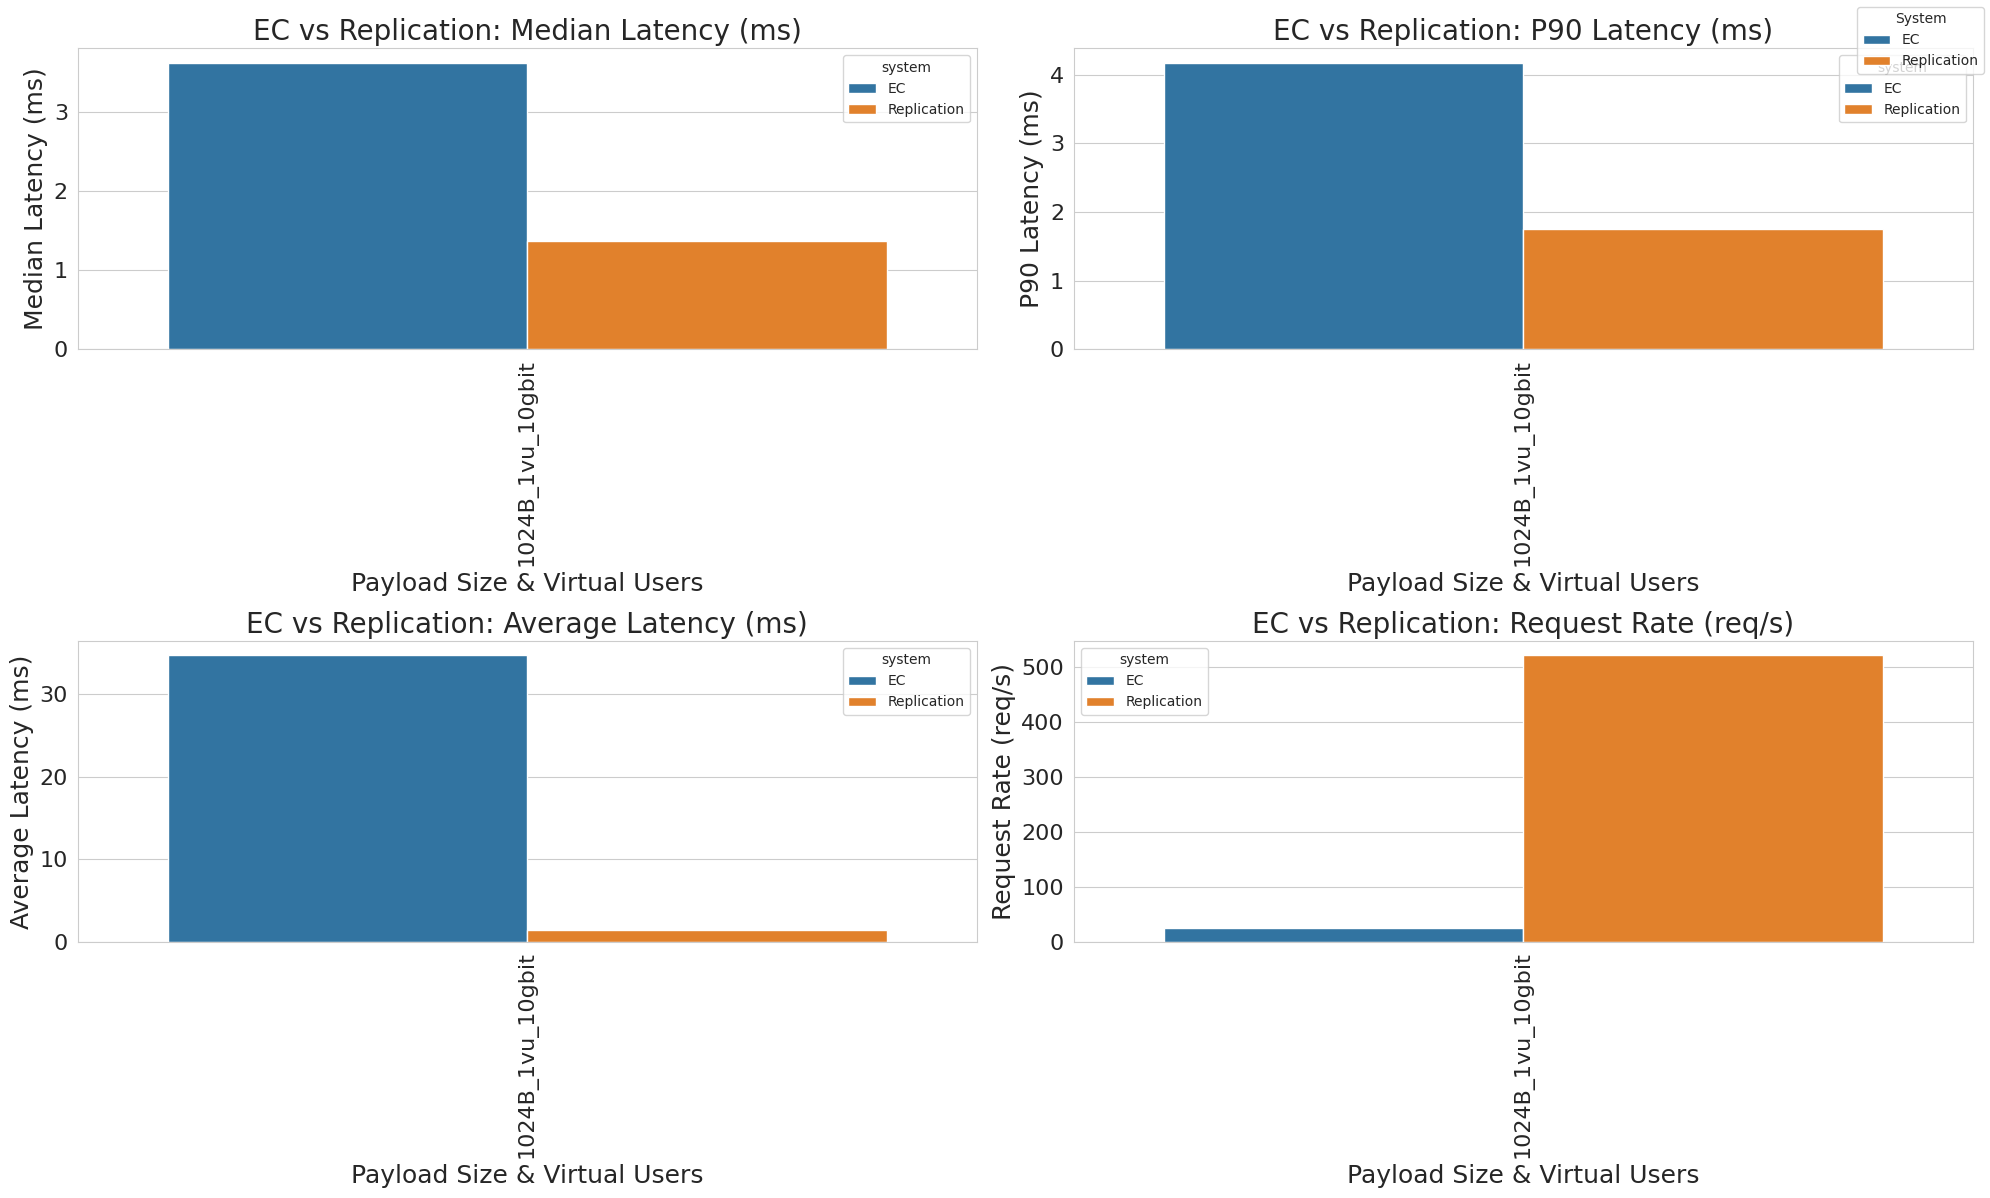
\includegraphics[width=0.8\textwidth]{resources/chapter-4/read_smload_fastnet.png}

    \caption{Kinerja Operasi Read pada Internet Cepat dan Payload Kecil}
    \label{fig:read-smload-fastnet}
  \end{figure}

  Proses \textit{erasure coding} memerlukan rekonstruksi data sehingga kinerjanya selalu lebih lambat dibandingkan replikasi. Grafik tersebut memperlihatkan kinerja \textit{erasure coding} dan replikasi memiliki perbedaan yang signifikan.

  \item Skenario 2: Internet lambat dan \textit{payload} besar
  
  Skenario kedua berlawanan dengan skenario pertama pada operasi \textit{write}. Namun, kondisi ini tidak berlaku untuk operasi \textit{read}. Gambar \ref{fig:read-bigload-slownet} menunjukkan hasil \textit{benchmark} untuk skenario ini.

  \begin{figure}[ht]
    \centering
    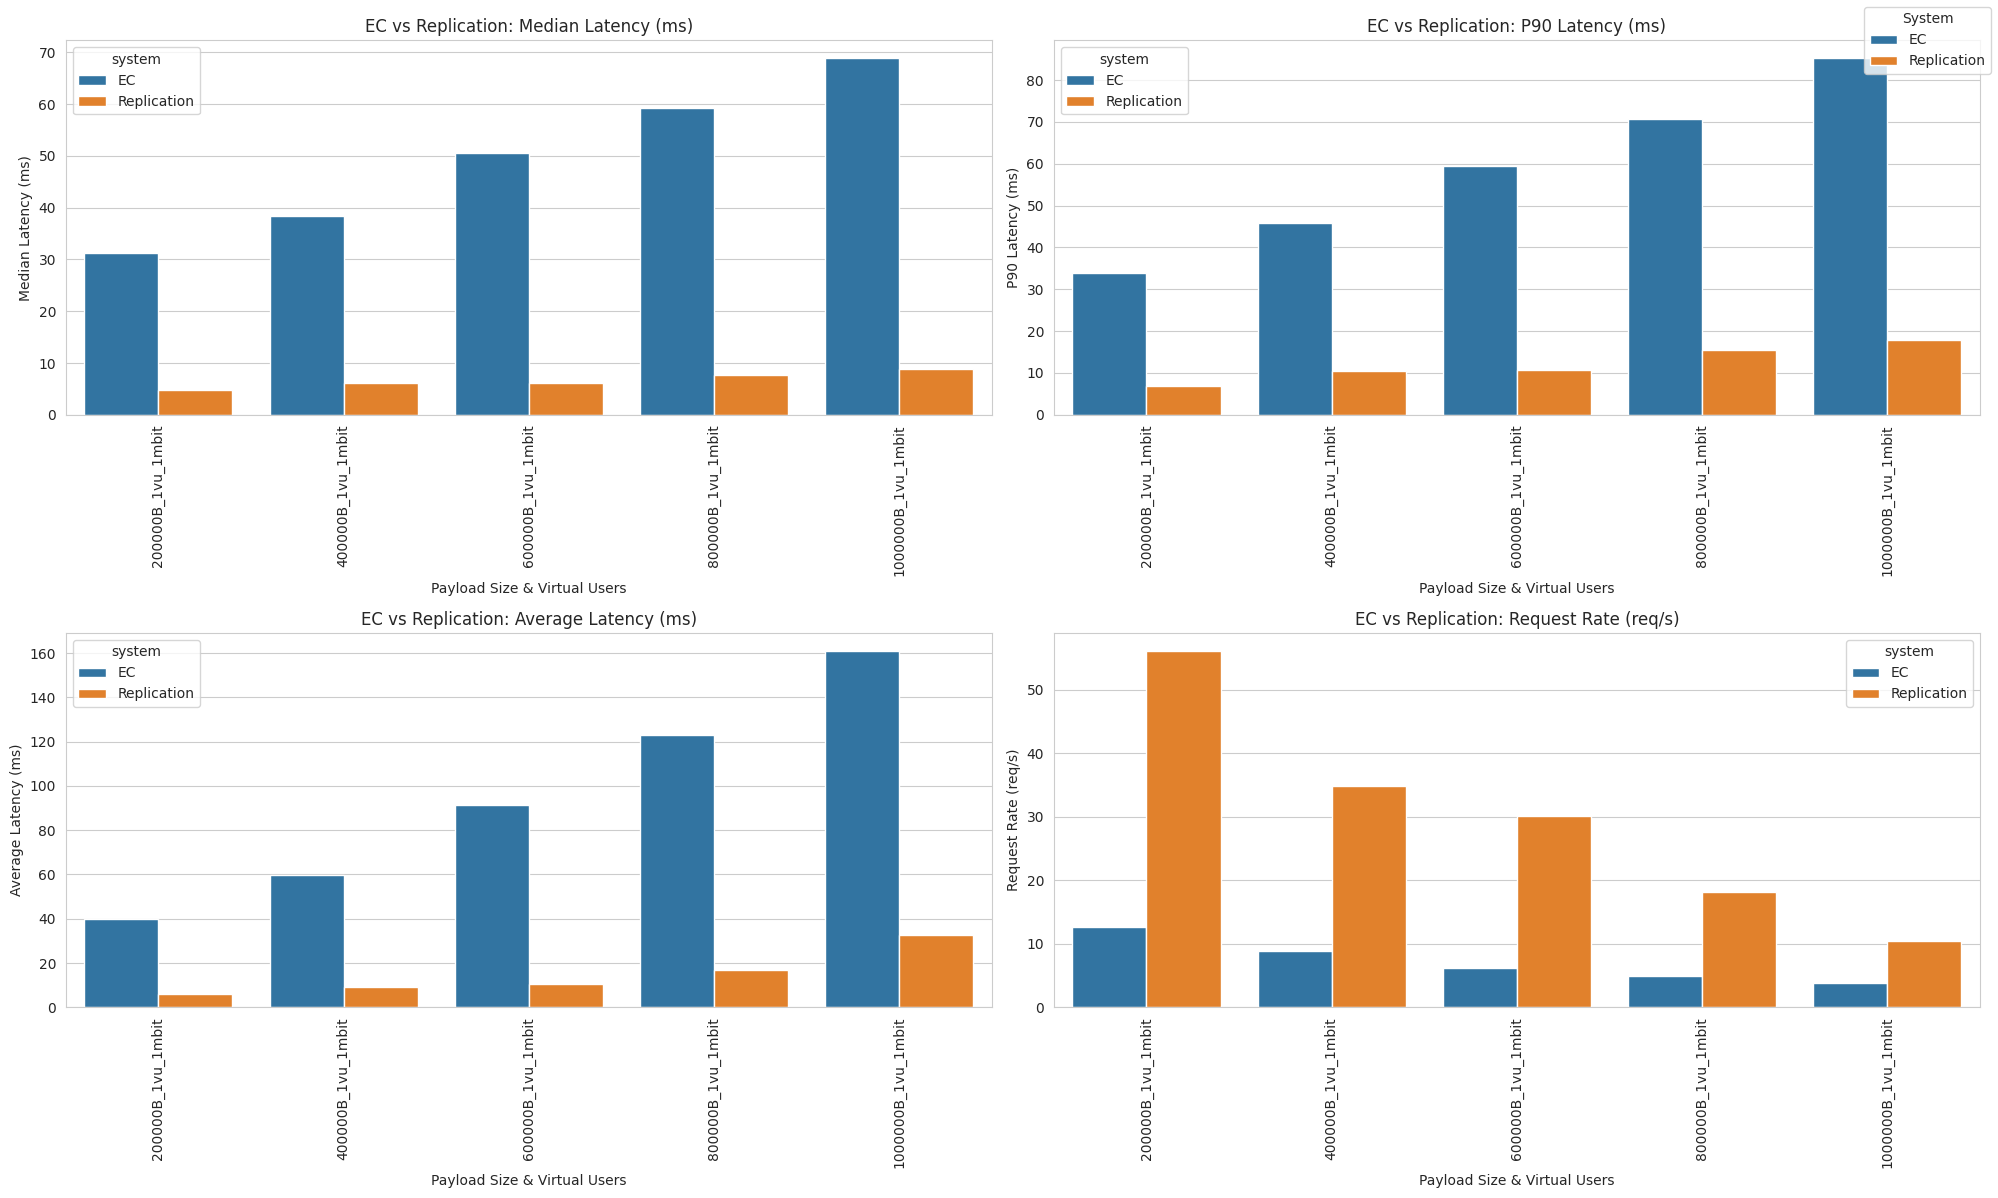
\includegraphics[width=0.8\textwidth]{resources/chapter-4/read_bigload_slownet.png}

    \caption{Kinerja Operasi Read pada Internet Lambat dan Payload Besar}
    \label{fig:read-bigload-slownet}
  \end{figure}

  Hasil dari skenario ini mengkonfirmasi bahwa \textit{erasure coding} tidak dapat mengungguli replikasi dalam kondisi apapun untuk operasi \textit{read}. Proses rekonstruksi data pada sistem \textit{erasure coding} akan tetap membutuhkan waktu yang lebih lama dibandingkan dengan replikasi, meskipun dalam kondisi internet lambat dan \textit{payload} besar. Selain itu, hasil ini menunjukkan juga bahwa keuntungan yang dimiliki \textit{erasure coding} dalam operasi \textit{write} perlu diiringi dengan penurunan kinerja pada operasi \textit{read}.

  \item Skenario 3: Internet menengah dan \textit{payload} besar
  
  Dari konfirmasi yang didapatkan dari kedua skenario sebelumnya bahwa \textit{erasure coding} tidak dapat mengungguli replilkasi untuk operasi \textit{read} dalam kondisi apapun, skenario ketiga melakukan eksplorasi tambahan terkait signifikansi perbedaan kinerja antar \textit{erasure coding} dan replikasi. Gambar \ref{fig:read-bigload-avgnet} menunjukkan hasil \textit{benchmark} untuk skenario ini.

  \begin{figure}[ht]
    \centering
    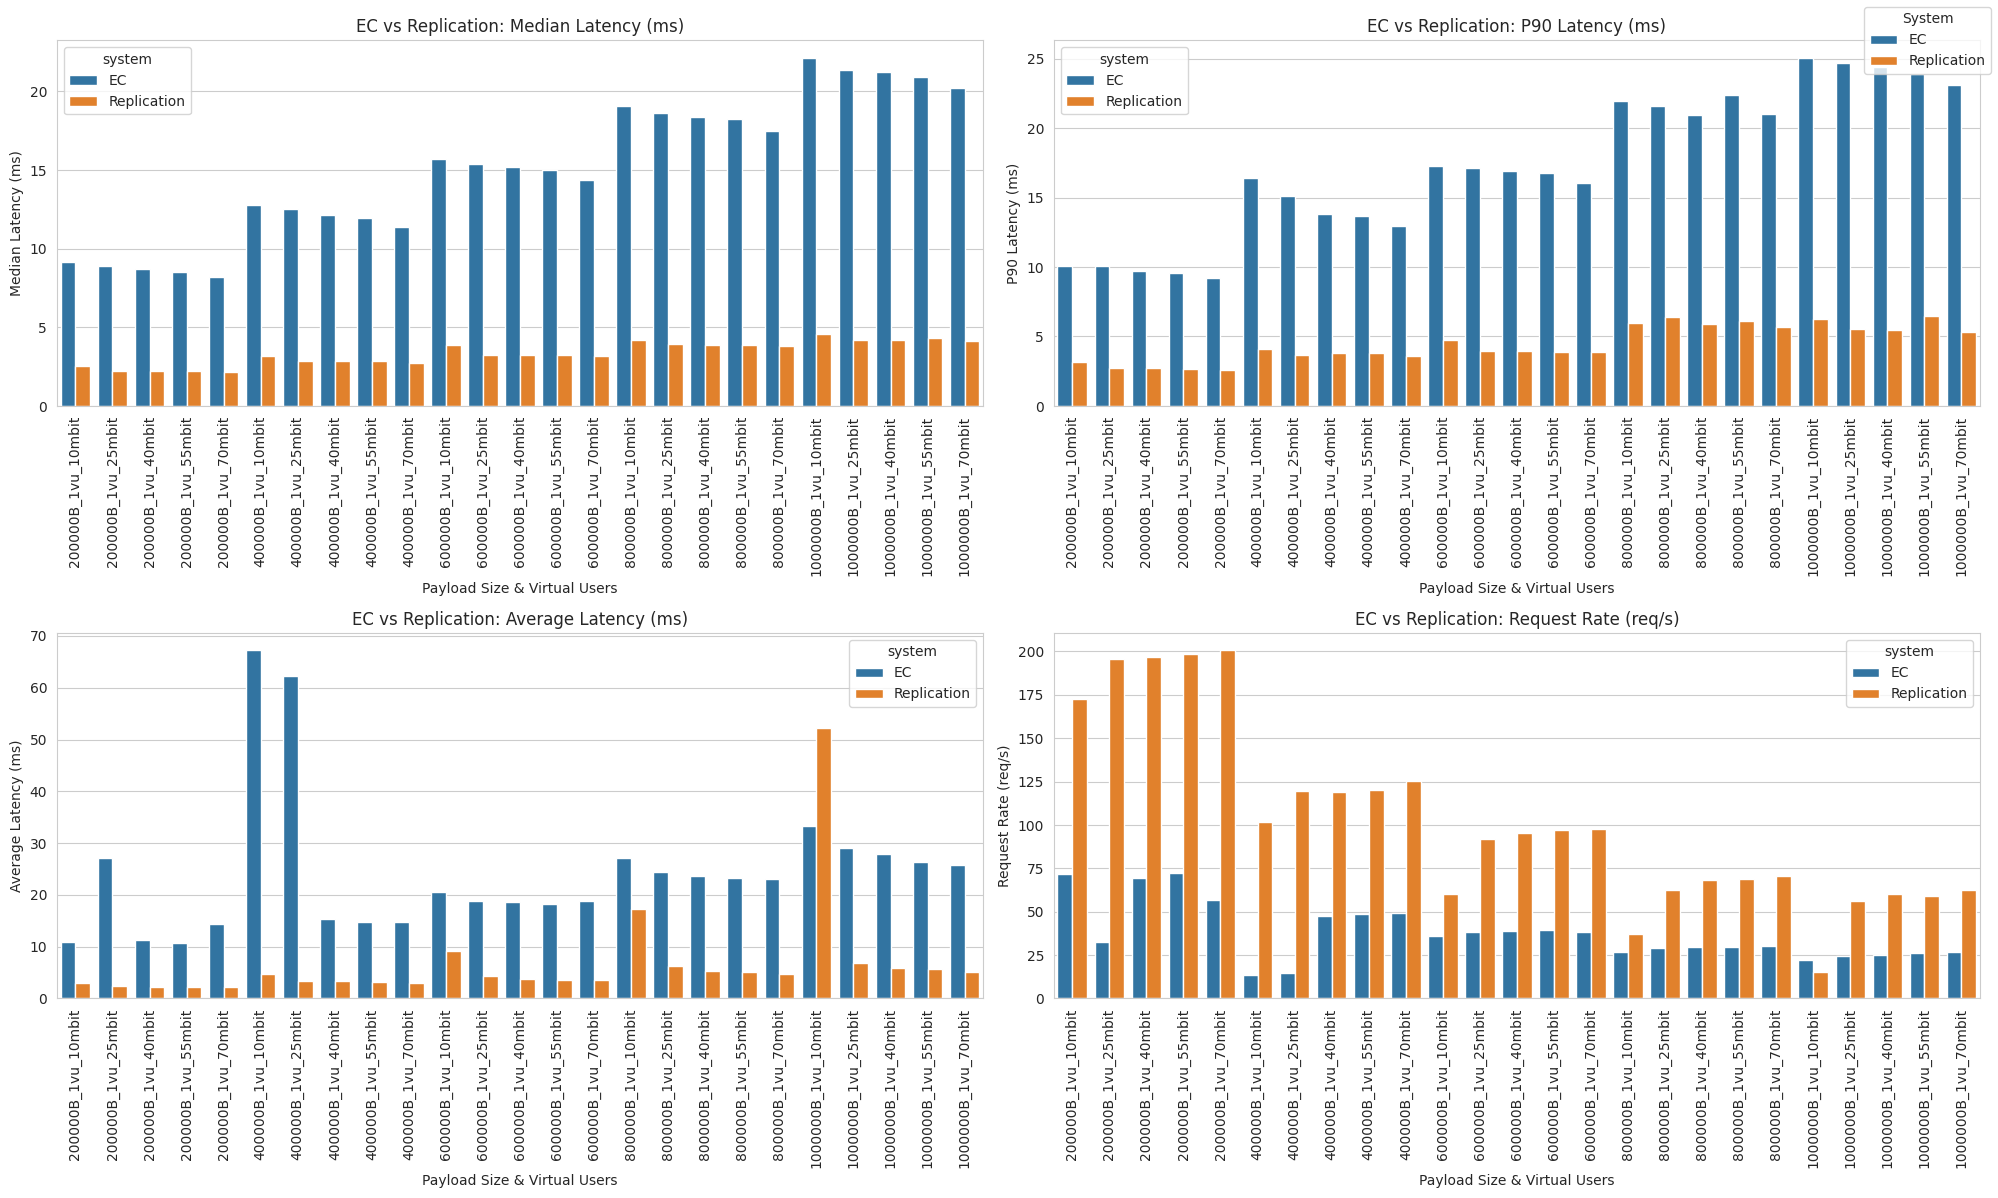
\includegraphics[width=0.8\textwidth]{resources/chapter-4/read_bigload_avgnet.png}

    \caption{Kinerja Operasi Read pada Internet Menengah dan Payload Besar}
    \label{fig:read-bigload-avgnet}
  \end{figure}

  Mengabaikan data \textit{noise} hasil \textit{benchmark}. Grafik tersebut menunjukkan perbedaan kinerja antara sistem berbasis \textit{erasure coding} dan replikasi secara umum menurun dengan \textit{payload} yang lebih kecil. Hal ini disebabkan oleh proses rekonstruksi data berjalan lebih cepat ketika \textit{payload} yang direkonstruksi lebih kecil dengan berkurangnya operasi yang perlu dilakukan dan juga pengiriman data antar-\textit{node}.

  Visualisasi \textit{heatmap} pada Gambar \ref{fig:read-bigload-avgnet-heatmap} menunjukkan perbedaan kinerja replikasi unggul pada operasi \textit{read}. Keunggulan ini semakin bertambah ketika \textit{payload} yang direkonstruksi semakin besar. Perubahan \textit{bandwidth} juga mempengaruhi kinerja \textit{erasure coding} dan replikasi. Penambahan \textit{bandwidth} menambah \textit{response time} dari kedua sistem, namun \textit{erasure coding} terlihat lebih terpengaruh dibandingkan replikasi. Hal ini disebabkan oleh proses rekonstruksi data yang membutuhkan pengumpulan \textit{fragment} dari beberapa \textit{node} terpisah terlebih dahulu melalui jaringan sebelum melakukan rekonstruksi, sedangkan replikasi hanya bertambah waktu yang diperlukan untuk mengirimkan data dari \textit{node} ke \textit{client}. Kode untuk visualisasi \textit{heatmap} dapat dilihat pada repository Github hasil implementasi.

  \begin{figure}[ht]
    \centering
    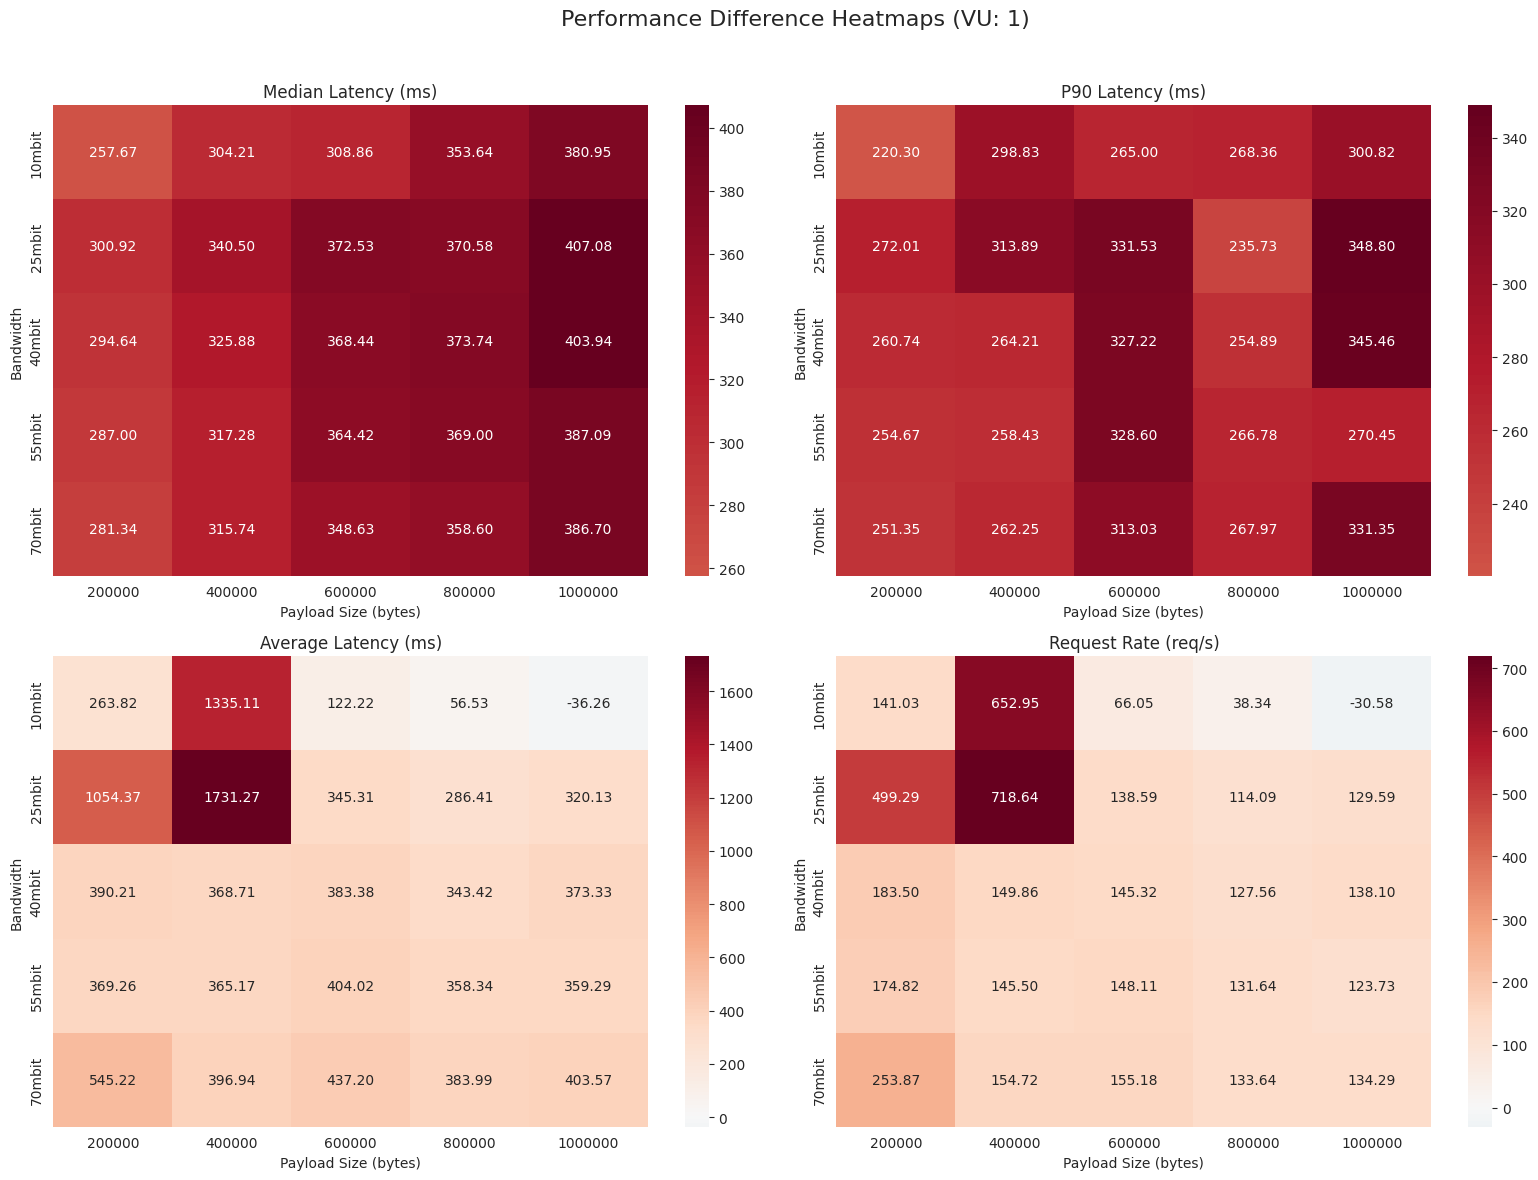
\includegraphics[width=0.8\textwidth]{resources/chapter-4/read_bigload_avgnet_heatmap.png}

    \caption{Heatmap Read pada Internet Menengah dan Payload Besar}
    \label{fig:read-bigload-avgnet-heatmap}
  \end{figure}

  Jike dibentuk diagram garis untuk memvisualisasikan pendekatan kinerja operasi \textit{read} pada sistem berbasis \textit{erasure coding} dan replikasi. Terlihat bahwa diagram garis yang dibentuk tidak menunjukkan \textit{trajectory} bahwa garis akan bersinggungan dengan garis \textit{erasure coding} pada titik tertentu. Perbandingan kinerja replikasi dan \textit{erasure coding} pada operasi \textit{read} memiliki kurva yang berbeda dan tidak akan bersinggungan. Diagram garis ini dapat dilihat pada Gambar \ref{fig:read-bigload-avgnet-line}.

  \begin{figure}[ht]
    \centering
    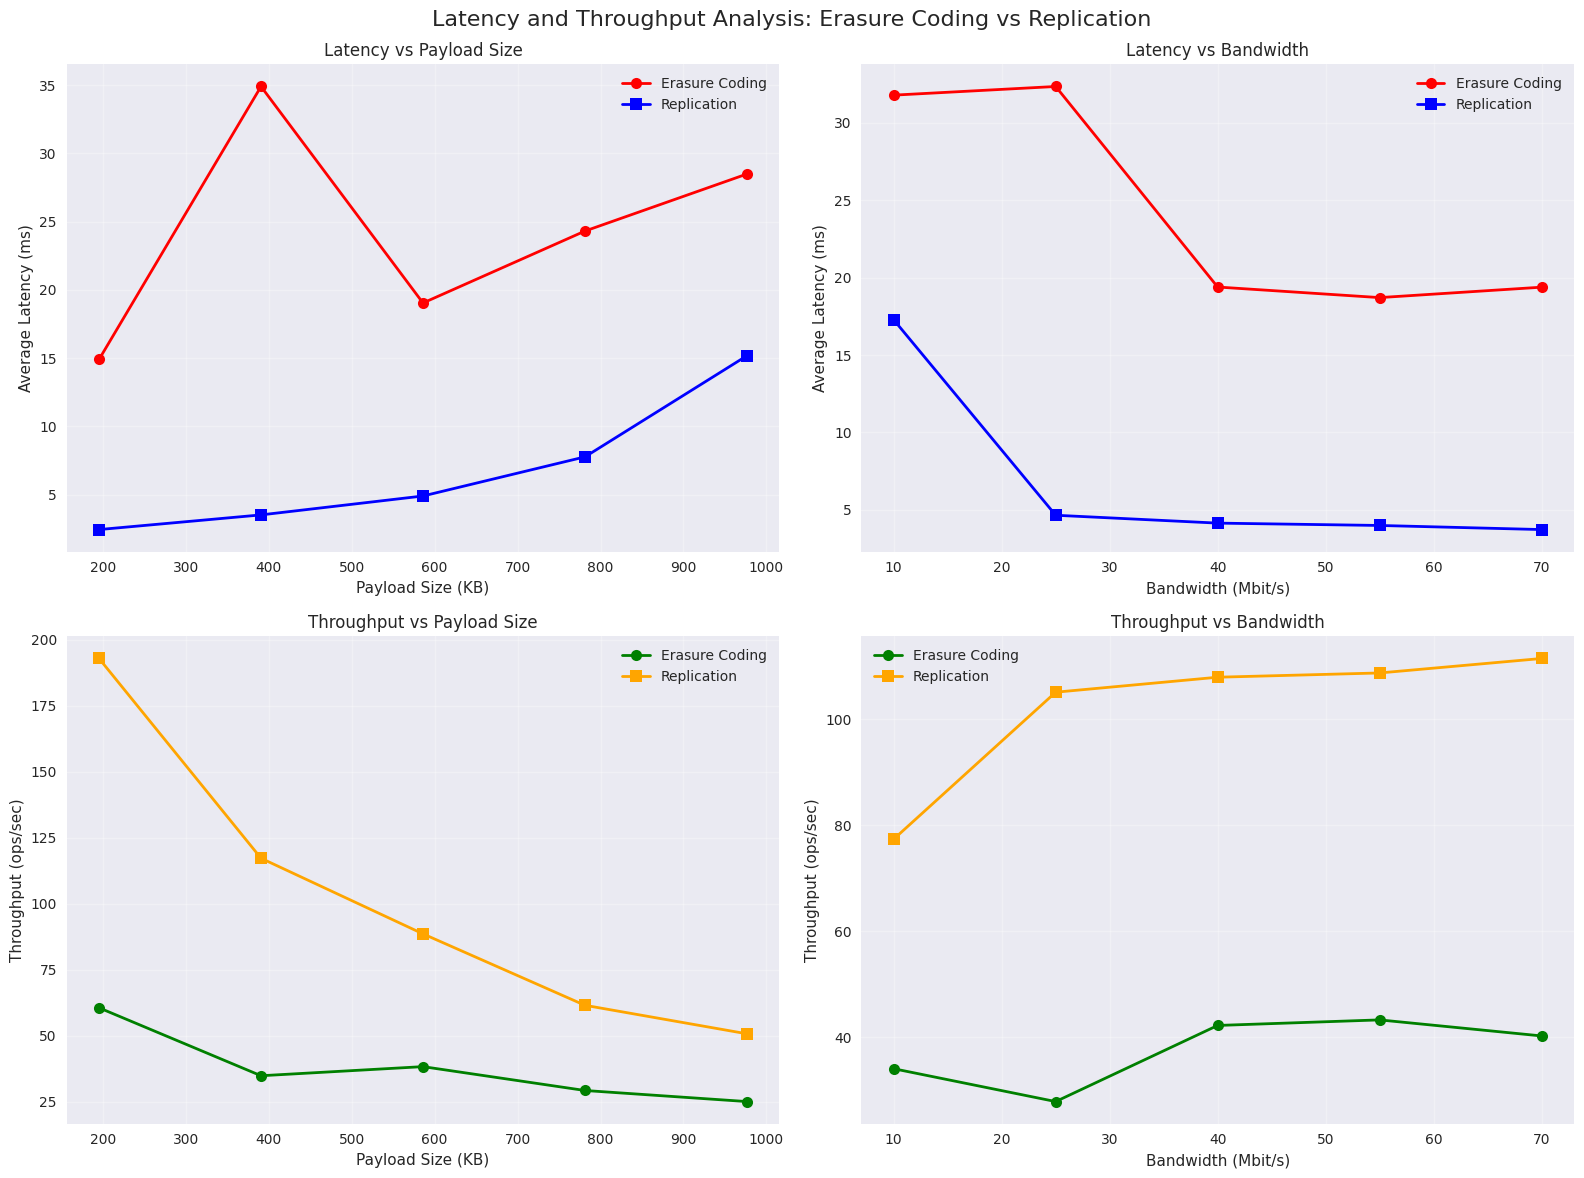
\includegraphics[width=0.8\textwidth]{resources/chapter-4/read_bigload_avgnet_line.png}

    \caption{Diagram Garis Read pada Internet Menengah dan Payload Besar}
    \label{fig:read-bigload-avgnet-line}
  \end{figure}

  Pembuktian matematis sederhana dapat dilakukan untuk menyatakan bahwa kinerja \textit{erasure coding} tidak akan pernah mengungguli replikasi pada operasi \textit{read}. Erasure coding akan membutuhkan waktu untuk memberikan data pada \textit{client}, rekonstruksi, dan meminta \textit{shard} pada \textit{node} lainnya, sedangkan replikasi hanya membutuhkan waktu untuk memberikan data pada \textit{client}. Persamaan \ref{eq:ec-read-latency} dan Persamaan \ref{eq:rep-read-latency} menunjukkan perhitungan latensi operasi \textit{read} pada sistem berbasis \textit{erasure coding}.

  \begin{align}
  L_{EC} &= T_{data} + T_{rekonstruksi} + T_{shard}
  \label{eq:ec-read-latency}
  \end{align}

  Sementara itu, Persamaan \ref{eq:rep-read-latency} menunjukkan perhitungan latensi operasi \textit{read} pada sistem berbasis replikasi.

  \begin{align}
  L_{REP} &= T_{data}
  \label{eq:rep-read-latency}
  \end{align}

  Dari persamaan tersebut, waktu antara \textit{erasure coding} dan replikasi dapat dituliskan sebagai Persamaan \ref{eq:read-latency-diff}.

  \begin{align}
  \Delta L &= L_{EC} - L_{REP} \\
  &= (T_{data} + T_{rekonstruksi} + T_{shard}) - T_{data} \\
  &= T_{rekonstruksi} + T_{shard}
  \label{eq:read-latency-diff}
  \end{align}

  Dengan demikian, perbedaan waktu antara \textit{erasure coding} dan replikasi akan menjadi semakin besar relatif terhadap ukuran data ketika data direkonstruksi, ukuran data ketika pengiriman data, dan juga \textit{bandwidth} yang tersedia ketika pengiriman data.
  
  Penambahan \textit{in-memory store} akan menghilangkan penambahan waktu ini. Namun, tidak semua \textit{request} dapat dilayani menggunakan \textit{in-memory store} karena keterbatasan memory yang tersedia. Oleh karena itu, peningkatan kinerja \textit{in-memory store} relatif terhadap rasio \textit{hit} dan \textit{miss} dari \textit{key} yang diminta. Jika \textit{hit} adalah seratus persen, maka \textit{erasure coding} akan memiliki kinerja yang setara dengan replikasi. Penambahan \textit{in-memory store} memodifikasi Persamaan \ref{eq:ec-read-latency} menjadi Persamaan \ref{eq:ec-read-latency-inmemory}.

  \begin{align}
    L_{EC} &= T_{data} + (T_{rekonstruksi} + T_{shard}) \times (1 - \text{hit rate})
    \label{eq:ec-read-latency-inmemory}
  \end{align}

  Dari persamaan tersebut, penambahan waktu yang dibutuhkan untuk operasi \textit{read} pada sistem berbasis \textit{erasure coding} dapat dihitung dengan mengurangi waktu yang dibutuhkan untuk operasi \textit{read} pada sistem replikasi. Persamaan ini dapat dituliskan sebagai Persamaan \ref{eq:ec-read-latency-diff-inmemory}.

  \begin{align}
    \Delta L &= L_{EC} - L_{REP} \\
    &= \left[T_{data} + (T_{rekonstruksi} + T_{shard}) \times (1 - \text{hit rate})\right] - T_{data} \\
    &= (T_{rekonstruksi} + T_{shard}) \times (1 - \text{hit rate})
    \label{eq:ec-read-latency-diff-inmemory}
  \end{align}

  Penambahan \textit{in-memory store} akan mengurangi waktu operasi \textit{read} pada sistem berbasis \textit{erasure coding} dengan kemungkinan untuk mengimbangi kinerja replikasi. Namun, hal ini tergantung pada rasio \textit{hit} yang dapat dicapai oleh \textit{in-memory store}.
  
  % Jika analisis regresi yang mirip dengan analisis pada Bagian \ref{subsubsection:analisis-operasi-write} dilakukan, hasil menunjukkan bahwa untuk semua skenario, \textit{erasure coding} memiliki kinerja yang lebih lambat dibandingkan replikasi. Grafik akhir dari analisis ini dapat dilihat pada Gambar \ref{fig:read-bigload-avgnet-regression}. Perlu diamati juga bahwa nilai \textit{R-squared} yang didapatkan dari analisis regresi ini adalah ada di bawah 0.5, yang menunjukkan bahwa model regresi ini tidak dapat menjelaskan variasi data dengan baik. Hal ini sebagian besar disebabkan oleh adanya \textit{noise} yang tinggi pada hasil \textit{benchmark}.

  % \begin{figure}[ht]
  %   \centering
  %   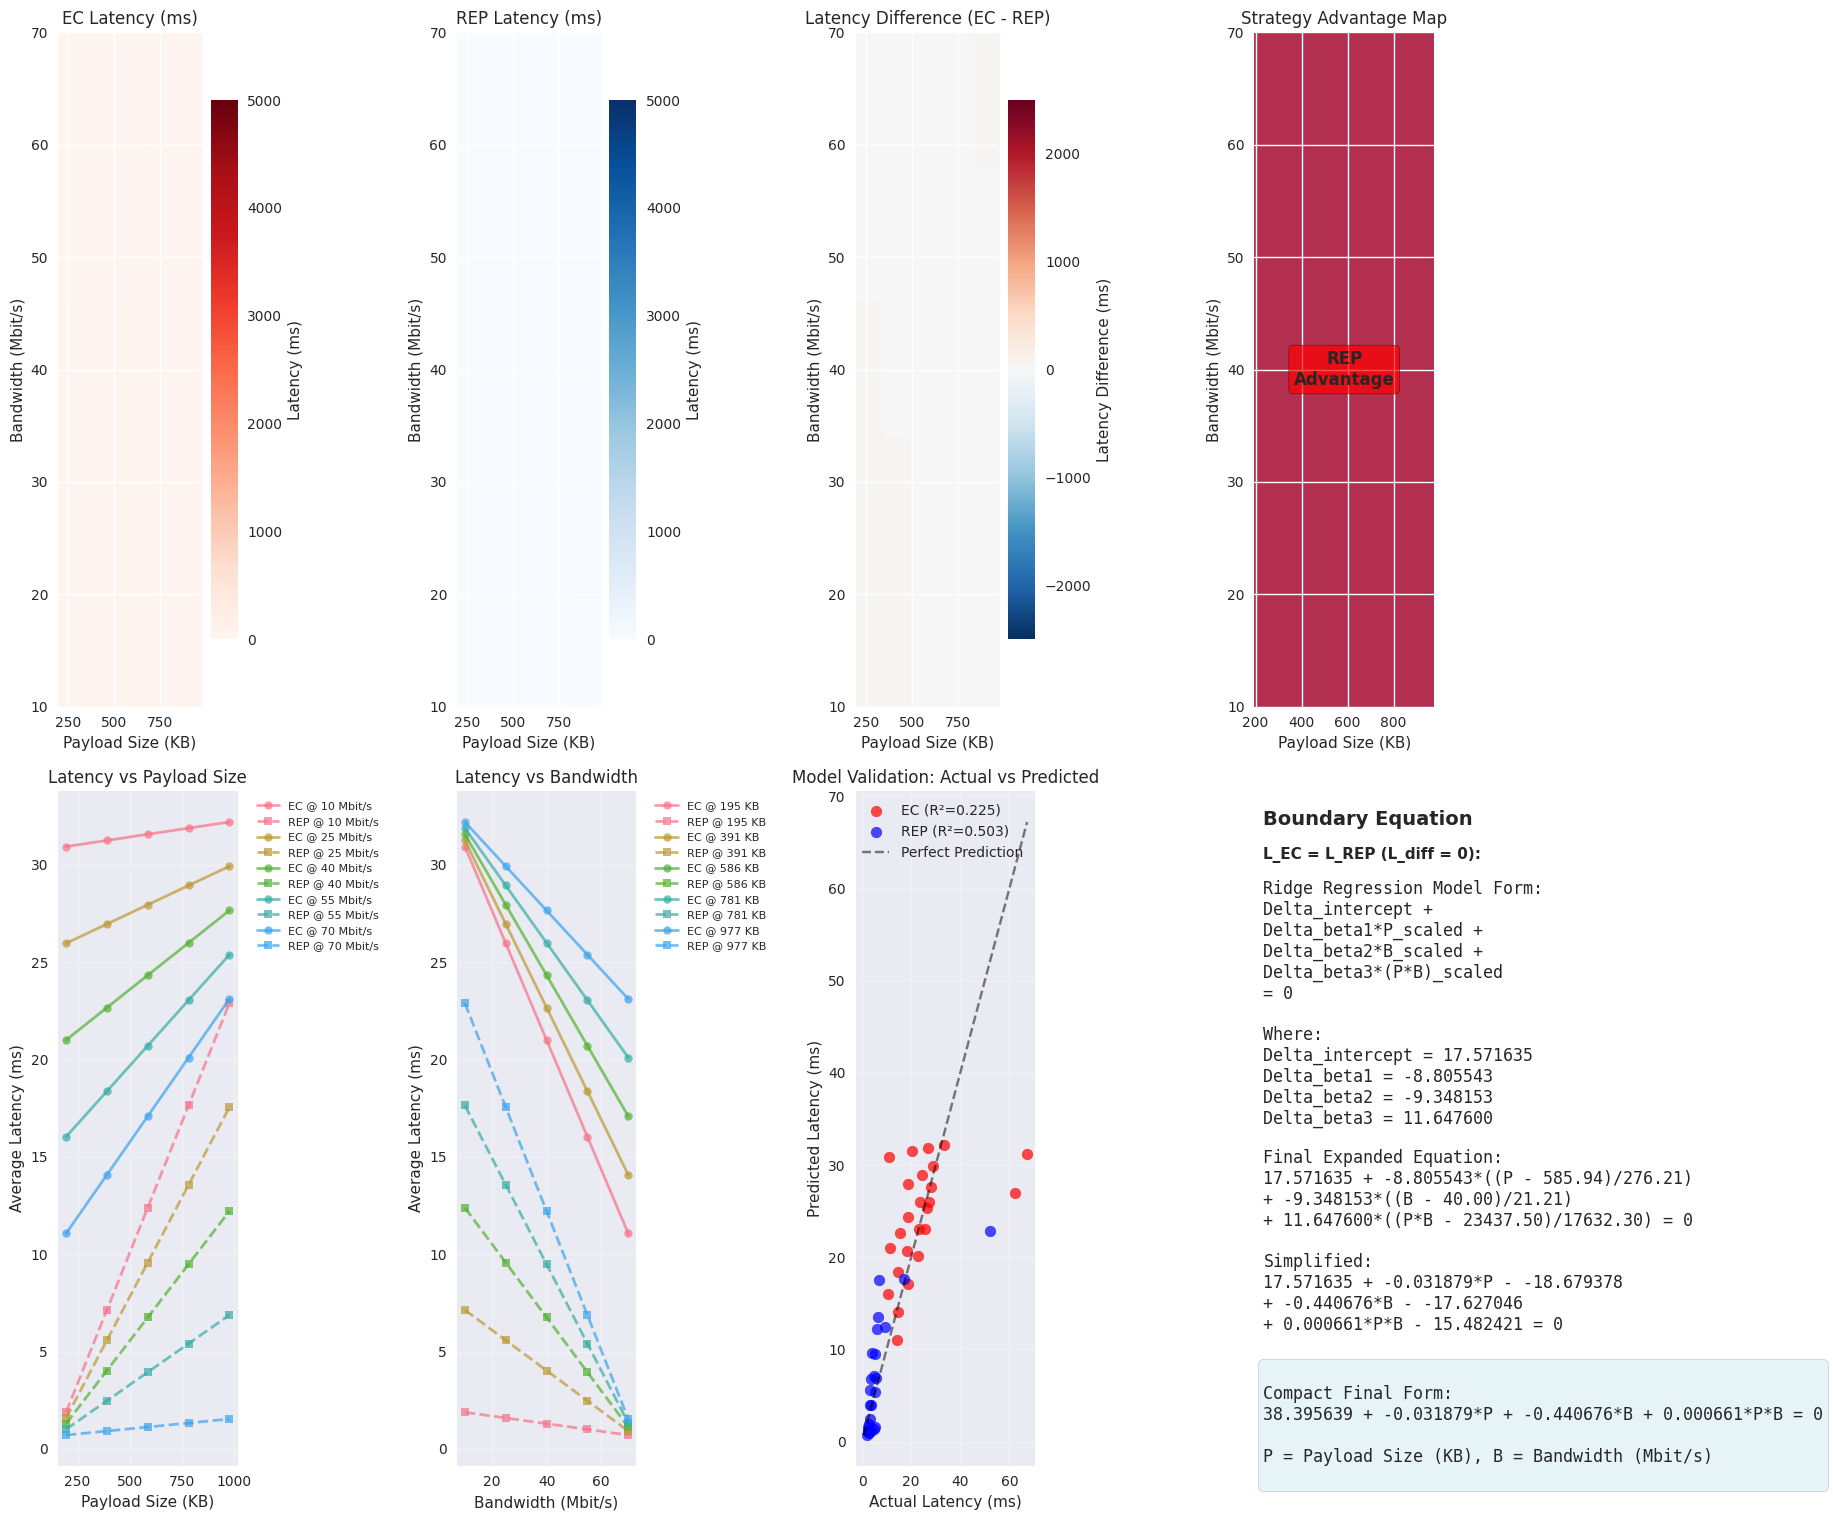
\includegraphics[width=0.8\textwidth]{resources/chapter-4/read_bigload_avgnet_regression.png}

  %   \caption{Analisis Regresi Read pada Internet Menengah dan Payload Besar}
  %   \label{fig:read-bigload-avgnet-regression}
  % \end{figure}
\end{enumerate}